\documentclass{homework}

\title{02MECHZ - Final \\ 03.02.2023}
%\author{I. Yalcinkaya}

\date{\vspace{-11ex}}

\begin{document}

\maketitle

\exercise

\begin{figure}[h]
\centering
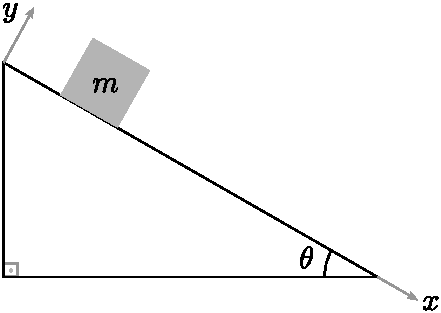
\includegraphics[scale=1.]{figures/q1.pdf}
\end{figure}

A block of mass $m$ sliding down on an inclined plane with an inclination angle $\theta$ and kinetic friction coefficient $\mu_k$
\begin{itemize}
    \item [\textbf{(a)}] Draw the free-body diagram of the block.
    \item[\textbf{(b)}] Write down Newton's second law for y-direction in magnitude form in terms of $N$, $m$,  $g$ (gravitational constant), and $\theta$.
    \item[\textbf{(c)}] Write down the magnitude of the frictional force acting in the block while it is sliding down in terms of $\mu_k$, $m$, $g$, and $\theta$.
    \item[\textbf{(d)}] Write down Newton's second law for x-direction in terms of $\ddot{x}$, $g$, $\theta$, and $\mu_k$.
    \item[\textbf{(e)}] Solve the differential equation (Newton's second law) you obtained in \textbf{(d)}, and find $x(t)$ for the initial conditions $x(0)=0$ and $\dot{x}(0)\equiv v(t)=0$.
    \item[\textbf{(f)}] Calculate the position of the block at $t=2~$s for $\theta=30^{\circ}$ ($g\approx 10~\text{m}/\text{s}^2$, $\sin 30^{\circ}=1/2$, $\cos 30^{\circ}=\sqrt{3}/2$, $\mu_k=\frac{1}{2\sqrt{3}}$)
\end{itemize}

\textit{Options from \textbf{(a)} to \textbf{(d)} are each worth 0.2 points. Options \textbf{(e)} to \textbf{(f)} are each worth 0.1 points - Total: 1 point} 

\exercise

\begin{figure}[h]
\centering
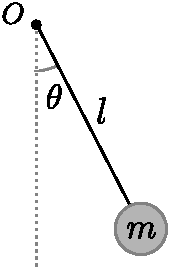
\includegraphics[scale=1.]{figures/q2.pdf}
\end{figure}

A simple pendulum of mass $m$ and length $l$ is swinging about its equilibrium point $\theta=0$.
\begin{itemize}
    \item[\textbf{(a)}] Draw the free body diagram of the mass.
    \item[\textbf{(b)}] What is the rotational inertia $I$ with respect to the hanging point $O$ in terms of $m$ and $l$?.
    \item[\textbf{(c)}] What is the torque $N$ acting on the mass with respect to point $O$ in terms of $l$, $m$, $g$, and $\theta$?
    \item[\textbf{(d)}] First write down the Newton's second law for rotations in terms of $N$, $I$, and $\alpha$ (angular acceleration $\ddot{\theta}\equiv \dot{\omega}\equiv \alpha$). Then, plug the results you found in \textbf{b} and \textbf{c} into Newton's second law. (Note: Be careful about signs)
    \item[\textbf{(e)}] Solve the differential equation (Newton's second law) you found in \textbf{d} to obtain $\theta(t)=Ae^{i\omega t}+Be^{-i\omega t}$ for small angle approximation $\theta \ll 1$. (Givens: $\sin\theta\approx \theta$ when $\theta\ll 1$, solution assumption: $\theta(t)=e^{\lambda t}$)
    \item[\textbf{(f)}] Given that $\theta(t)=Ae^{i\omega t}+Be^{-i\omega t}$ can be written as $\theta(t)=C\cos(\omega_0t)$, determine $C$ for the initial condition $\theta(0)=\theta_0$.
    \item[\textbf{(g)}] By using $\theta(t)$ with the initial condition $\theta(0)=\theta_0$, calculate the angular velocity of the pendulum $\omega=\dot{\theta}(t)$. At what time $t'$, $\dot{\theta}(t)$ does take its largest value (the maximum speed of the pendulum) for the first time after being released from rest? By using $\dot{\theta}(t')$ calculate the maximum value of the kinetic energy of the pendulum.
    \item[\textbf{(h)}] Calculate the maximum kinetic energy of the pendulum from the point of view of conservation of energy: Assume that mass $m$ has no potential energy at its equilibrium point ($\theta=0$). First calculate the potential energy then the pendulum is at rest ($\theta=\theta_0$). We know that this potential energy will completely be converted to pendulum's kinetic energy when $\theta=0$. (Given: $\cos\theta_0\approx 1-\theta_0^2/2$ for $\theta_0\ll 1$)
    \end{itemize}

\textit{Options from \textbf{(a)} to \textbf{(f)} are each worth 0.15 points. Options \textbf{(g)} to \textbf{(h)} are each worth 0.05 points - Total: 1 point} 

\exercise

Find the force law $f(r)$ for a central-force field that allows a particle to move in a spiral orbit given by $r=k\theta^2$, where $k$ is a constant. Given:

\begin{equation*}
    \dfrac{d^2}{d\theta^2}\left(\frac{1}{r}\right)+\frac{1}{r}=-\frac{\mu}{l^2}r^2f(r)
\end{equation*}
where $l$ is the angular momentum and $\mu$ is the reduced mass.


\textit{Total: 1 point} 

\exercise

\begin{figure}[h]
\centering
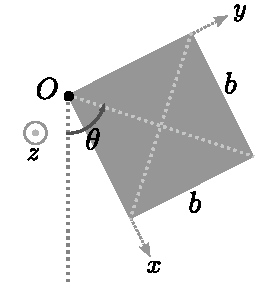
\includegraphics[scale=1]{figures/q4.pdf}
\end{figure}


A homogenous square plate with side length $b$ is hung from one of its corners $O$. The area density of the plate is $\rho_A=m/b^2$ where $m$ is the total mass of the plate. We assume that the plate is effectively two dimensional, i.e., there is no mass distribution in z direction.

\begin{itemize}
    \item[\textbf{(a)}] Calculate the inertia tensor $[\mathbf{I}]$ by using $I_{ij}=\int\rho(r)\left(\delta_{ij}\sum_k x_k^2-x_ix_j\right)$.
    \item[\textbf{(b)}]Calculate the angular momentum vector $\mathbf{L}$.
    \item[\textbf{(c)}]Calculate the magnitude of the torque $N$ applied on the center of mass of the square plate. 
    \item[\textbf{(d)}]Write down Newton's second law for rotations.
\end{itemize}

\textit{Each option is worth 0.4 points - Total: 1.2 point} 

\end{document}
